\documentclass[letterpaper, 10pt,titlepage]{article}

\usepackage{graphicx} 
\graphicspath{ {images/} }                                       
\usepackage{amssymb}                                         
\usepackage{amsmath}                                         
\usepackage{amsthm}                                          
\usepackage{alltt}                                           
\usepackage{float}
\usepackage{color}
\usepackage{url}
\usepackage[letterpaper, margin=0.75in]{geometry}
\usepackage{enumitem}
\usepackage{pstricks, pst-node}
\usepackage{hyperref}
\usepackage[utf8]{inputenc}
\usepackage{underscore}
 \usepackage{url}
\hypersetup{
  colorlinks = true,
  linkcolor  = black
}

\setcounter{secnumdepth}{4}
\def\name{Chongxian Chen}

\hypersetup{
  colorlinks = true,
  urlcolor = black,
  pdfauthor = {\name},
  pdfkeywords = {Problem Statement},
  pdftitle = {Capstone Project},
  pdfsubject = {Capstone Project},
  pdfpagemode = UseNone
}

\renewcommand*\contentsname{Table of Contents}


\begin{document}

\begin{center}

Oregon State University Computer Science Senior Design Winter 2016
\bigbreak
Progress Report
\bigbreak
By Alex Hoffer, Jake Smith, and Chen Chongxian
\bigbreak
Team Name: Stat Champs
\bigbreak
\vspace{3.0cm}
Abstract
\bigbreak
The application of machine learning to Biochemistry and Biophysics has enabled researchers in this field to make remarkable discoveries, such as the generation of new DNA sequences. However, students of Biochemistry and Biophysics do not get the opportunity to learn machine learning. Dr. Victor Hsu of the Oregon State University Biochemistry and Biophysics department has commissioned the Stat Champs to produce an instructional module to give his students the chance to familiarize themselves with machine learning. The software product the Stats Champs have agreed to develop is a web page that allows students to train a machine learning model based on the college basketball statistics and machine learning algorithm of their choosing in order to produce a March Madness bracket. This will help students understand how machine learning algorithms produce models and how inclusion or exclusion of certain data can influence such models. Over the course of Fall term 2016, the Stat Champs developed materials such as design documents and technology reviews in order to prepare for the engineering of the module. Then, in Winter term 2017, the Stat Champs began the software development phase of this project. This report comprehensively describes the progress thus made on this project, as of mid-February 2017.
\newpage
\end{center}

\tableofcontents

\newpage
\section{Introduction}
	This report chronicles the progress the Stat Champs have made on developing the machine learning instructional tool. In Fall term 2016, the progress that had been made was a project statement, a requirements document, a design document, a technology review, and a progress report. In Winter term 2017, the team made progress on the engineering of the module. The remaining sections of this report are devoted to each of the individual members of the Stat Champs to describe their experiences this term as well as their contributions to the software product.
\section{Progress Descriptions}
\subsection{Alex Hoffer}

\subsubsection{Project Purposes and Goals}
\par Our project was given to us by Dr. Victor Hsu of the Biochemistry and Biophysics department at Oregon State University. The purpose of this project is to demonstrate to Dr. Hsu's students how common machine learning algorithms generate models, and how the inclusion or exclusion of data can influence these models. Using an event like the March Madness tournament that produces binary outcomes (i.e. each team can only win or lose) facilitates the learning process by making the machine learned models easy to read, understand, and manipulate through the inclusion or exclusion of data. Thus, our goal is to help Dr. Hsu's students learn how machine learning works, and the degree to which our module is successful is predicted by whether or not the average student can begin to understand machine learning through our demonstration. 

\subsubsection{Brief recap of Alex's responsibilities}
\par As a team, we discussed each of our three responsibilities in Fall term 2016. My three responsibilities center around the graphical user interface (hereafter referred to as GUI) of the module. For me, the first responsibility was to host the web page and develop the general GUI to aid users in navigating the various sections of the website. Information pertaining to this first responsibility can be found in the subsection "Responsibility 1". Responsibility two was to present instructions on how to use the module before the machine learning module itself was presented. I have expanded this responsibility to include the development of two additional subsections of the site. These two additional, unplanned subsections are a Purpose page and an About page. These pages will be described in detail in the subsection "Responsibility 2", and my additions to my original second responsibility will be noted in a modified Technology Review document for the purpose of project documentation. My third responsibility was to take the data generated by Chongxian's machine learning algorithms and produce a March Madness bracket. More on the progress on this responsibility can be found in the section "Where Alex is Currently At in the Project". 
   
\subsubsection{Responsibility 1}
\par My first responsibility was to host the web page and develop the GUI for the project so that users can navigate through the website. Specifically, this responsibility consisted of four tasks. First, I hosted the website on my public_html folder that is provided to me by the Engineering department. Then, I had to produce HTML. That is, I had to construct the blueprints for what the site should look like. This consisted of things like a banner that contained links to different parts of the site, such as Home, Instructions, Module, Purpose, and About. Other than the banner, I added a title for the page to appear in the browser, the use of HTML divs, lists, sections, and other common tags to organize our website, which is just one big page, into logical chunks that correspond to the different features our website offers. While I established the parts of the site like Home, Instructions, etc., it was not until the second responsibility (which has its own section of this report dedicated to it) that I modified these in any way. My next task of this first responsibility was to produce CSS. Since my main motive in my contributions to this project were to ensure the usability of the module, it is only natural that I used CSS to customize the HTML tags. Without CSS, a website looks ugly. I added CSS that I believed would improve the user's experience with the website, because I felt that without a clean, readable interface, there would be unnecessary difficulties within the usage of the site that would hamper our target population's ability to learn machine learning. In other words, the hardest part to understand about this module should be the machine learning algorithms themselves, not the design that leads to using the module. The third task within this responsibility was to produce JavaScript. Without JavaScript, this page would be clunky and unresponsive. All moderately usable websites in our current era utilize JavaScript to make pages fun to use and to reduce the need for users to re-load the website to experience all features of the page, which serendipitiously also reduces the demand on the Engineering server the site is hosted on, which means more users can access our website at once. The specifics of the JavaScript contribution include making the individual items on the banner mentioned above light up when a mouse hovers over them, which helps keep the user informed about where they are in the web page. These list items located on the banner were also clickable, and when clicked, lead to the specific section of the page which its title referred to. This design decision was yet another opportunity to improve page usability by providing an intuitive way for users to navigate through the site, as well as reducing the load on the server by requiring fewer page refreshes. Therefore, the three technologies I required to fully implement this first responsibility were HTML, CSS, and JavaScript. The only problems I encountered in using these three technologies came from JavaScript, which I find to be a perplexing and complicated language. The use of JavaScript tutorials, programmer message boards, and documentation eased my woes in this dimension and enabled me to produce a GUI for our website that looks clean and understandable and is rewarding to interact with.

\includegraphics[width=\textwidth]{dv.jpg}
A screenshot image of the home page of our website. Images of each other section of the page can be found in the "Responsibility 2" section.

\subsubsection{Responsibility 2}
My second responsibility was to present instructions to the user on how to use the module before the module itself is presented. However, I expanded this responsibility after I developed the GUI in my first responsibility to encompass not only a section of the page devoted to the instructions, but also sections devoted to our purpose, about us, and the module itself. The instructions are thus far incomplete because we have not been able to get our machine learning module working (the responsibilities for the machine learning module functionality lie within other group mates' sections). There is currently a section of the page devoted to the module itself, which is also, given the incomplete status of the module, not occupied by anything meaningful. However, I have written the Purpose section (which encapsulates descriptions of this project's purpose that can be read in my section "Project Purposes and Goals", as well as the About Us section, which simply describes who we are and how to reach us if need be. The development of these sections was easy, since I merely built upon the GUI that I developed in my first responsibility. Therefore, through the combined magic of CSS and JavaScript I was able to produce a clean interface for all of these sections of our website. A particularly nice feature of note that was made possible by these two technologies is a button located at the bottom of each section that lit up when a mouse hovered over it and, if clicked, bounced the user on down to the next logical section of the website. The content of these sections can be found in images presented below.

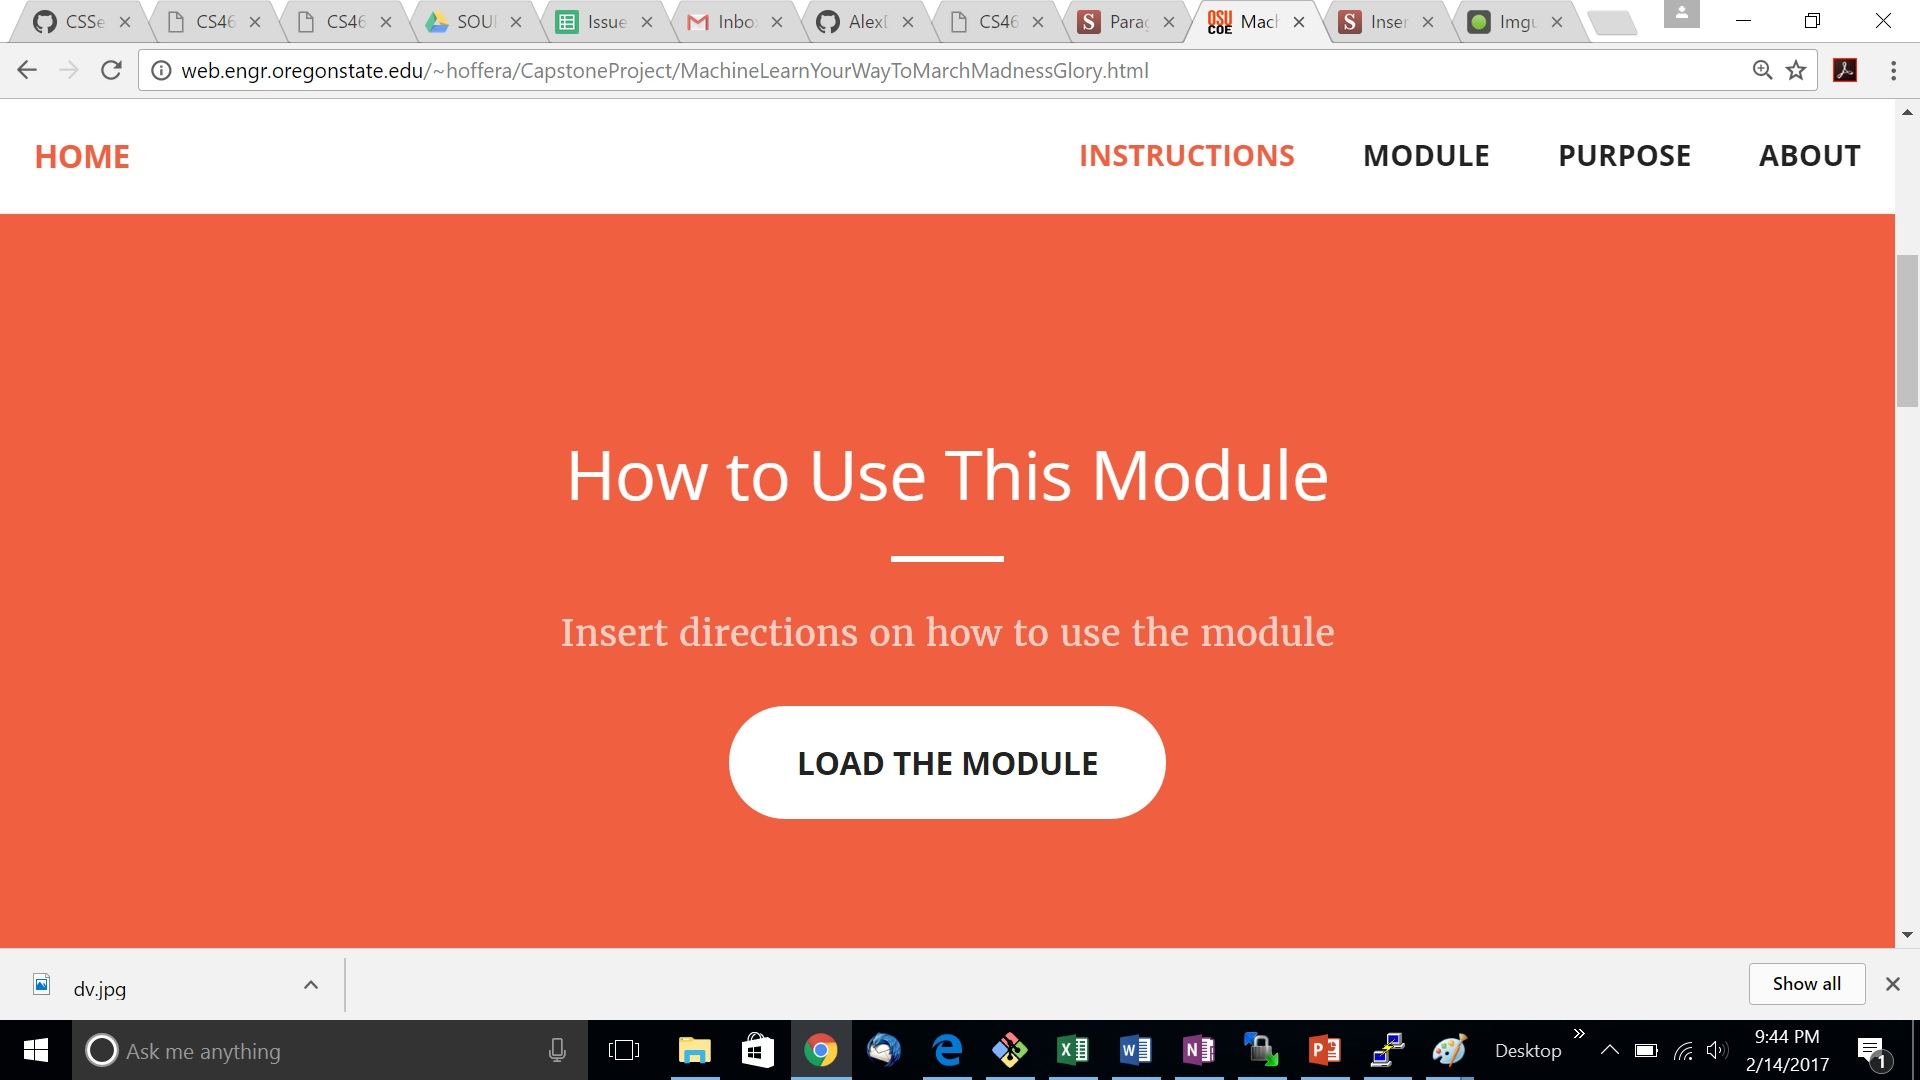
\includegraphics[width=\textwidth]{Instructions.jpg}
A screenshot image of the Instructions page of our website. Note that it remains incomplete until the module is created.

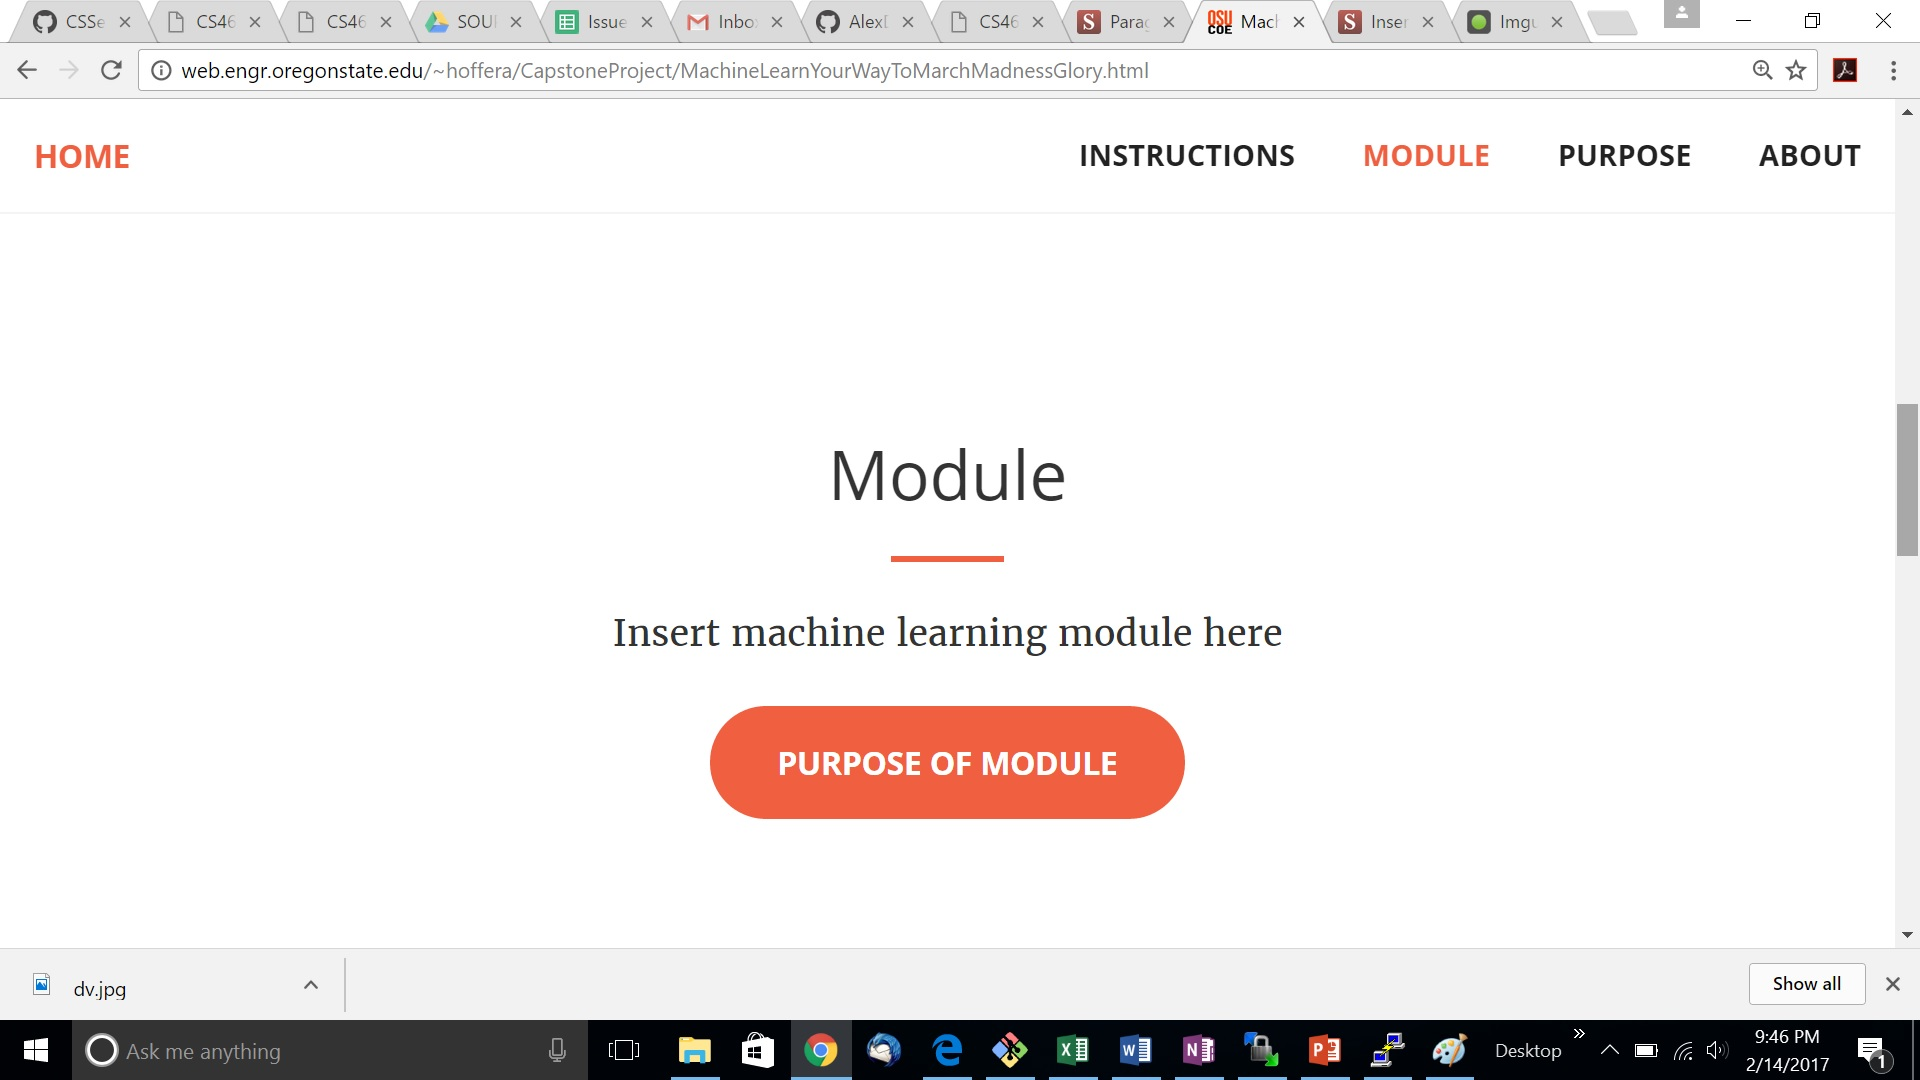
\includegraphics[width=\textwidth]{Module.jpg}
A screenshot image of the Module page. It awaits the completion of Chongxian's machine learning routines.

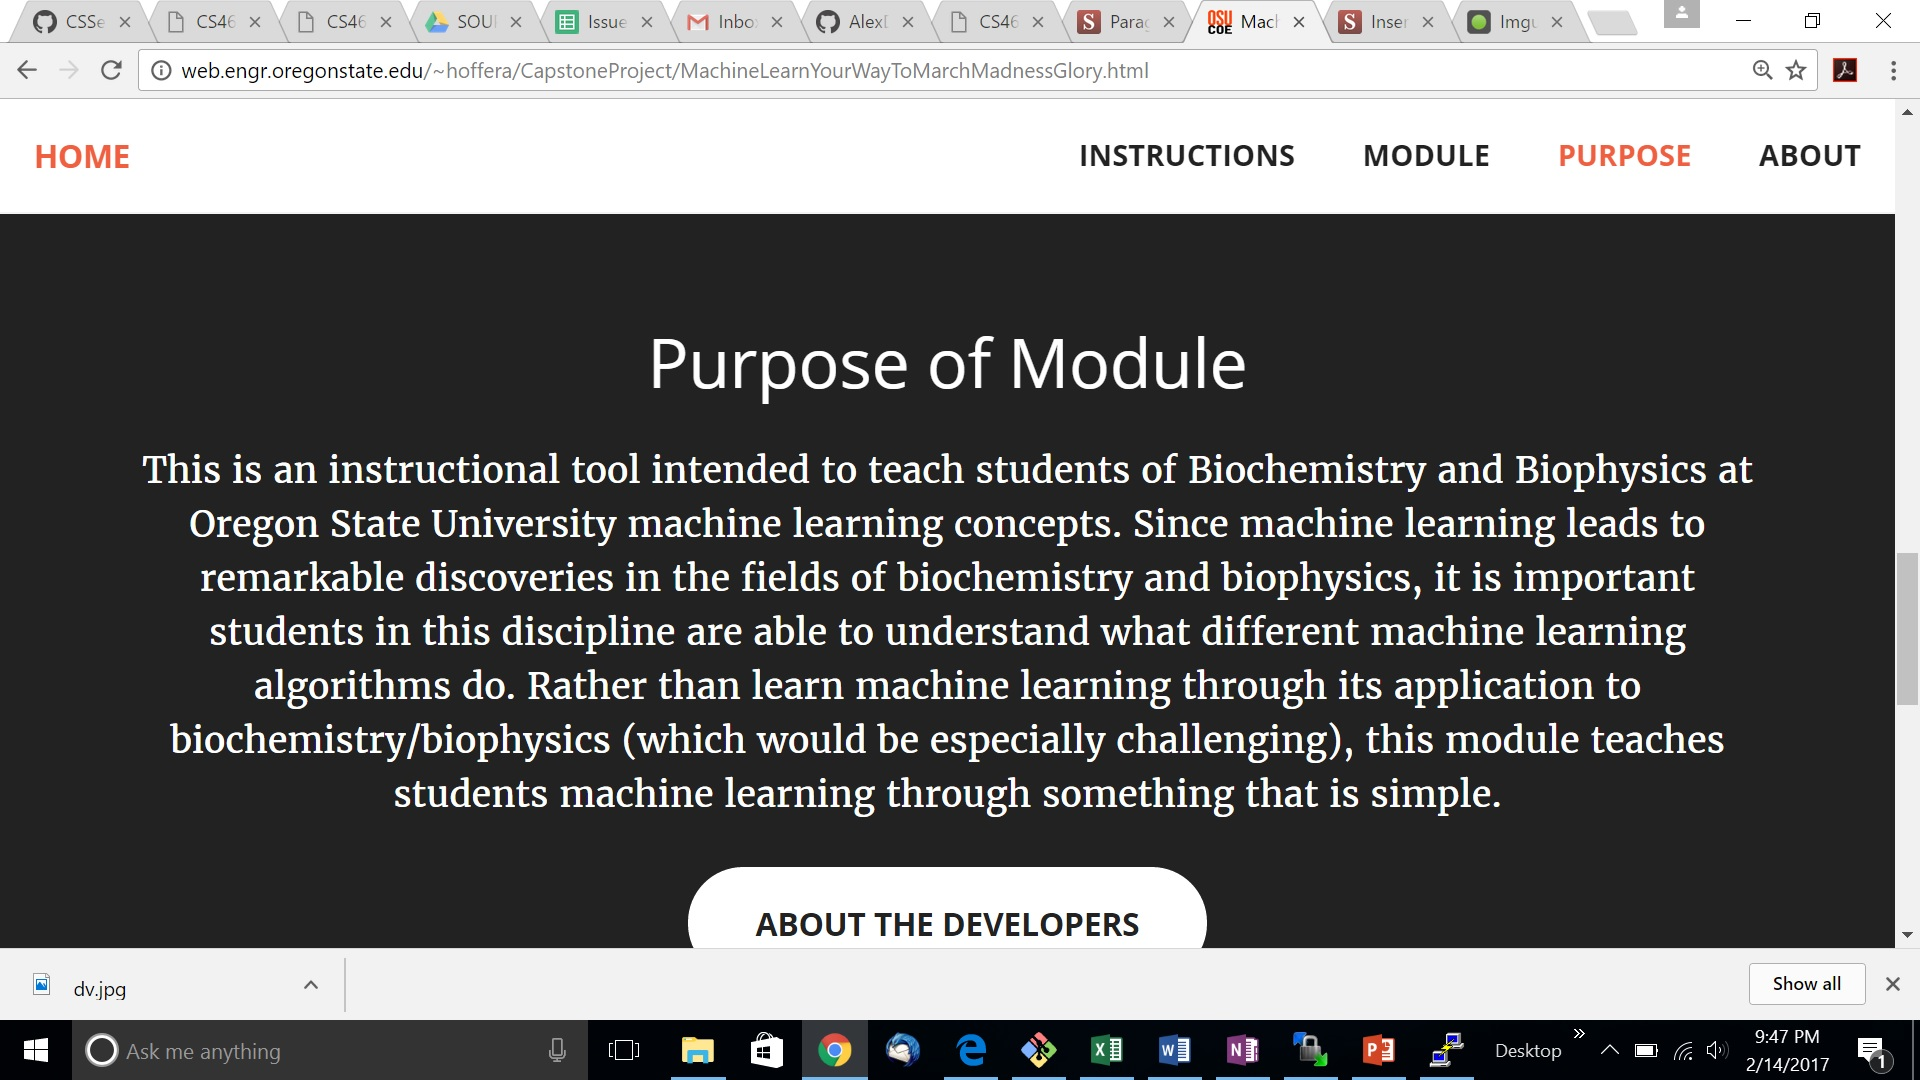
\includegraphics[width=\textwidth]{Purpose.jpg}
A screenshot image of the Purpose page, which describes why we are pursuing this project.

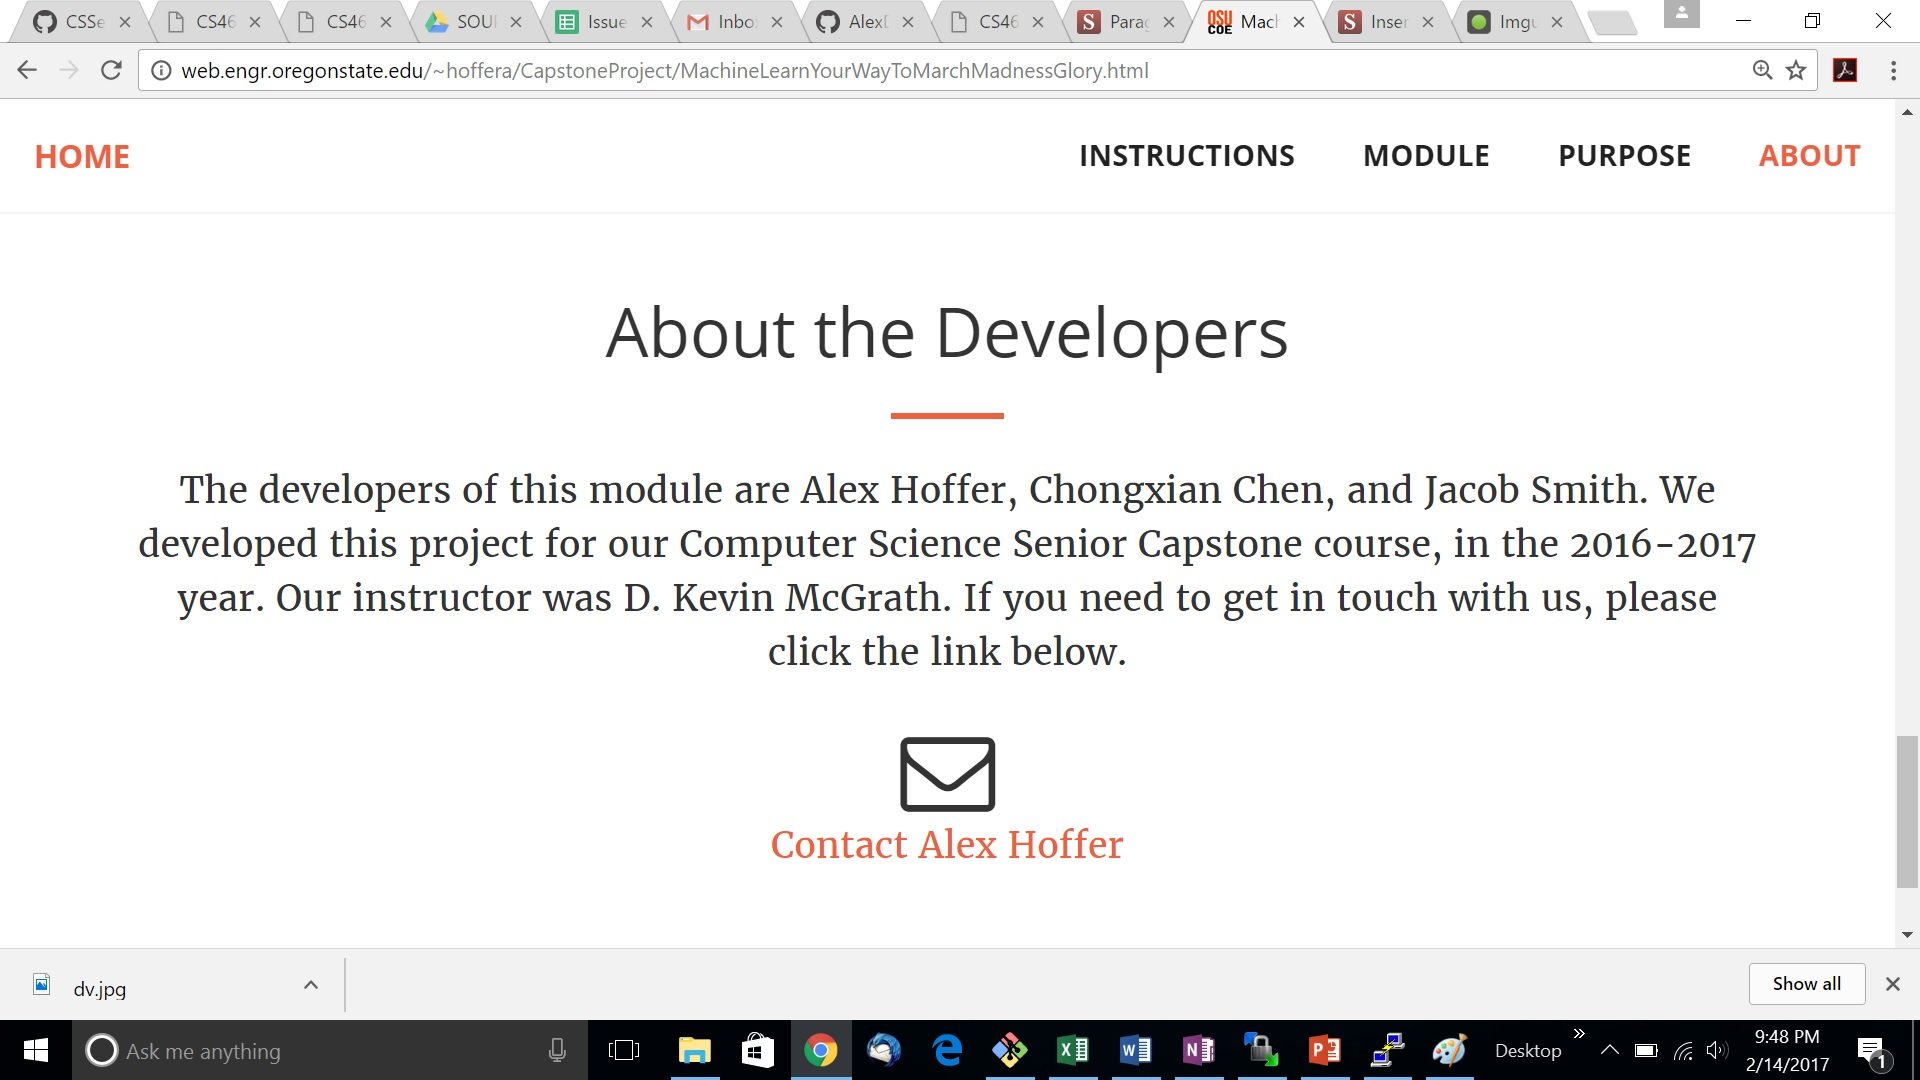
\includegraphics[width=\textwidth]{About.jpg}
A screenshot image of the About page, which describes who we are.

\subsubsection{Where Alex is currently at in the project}
\par I have two out of my three responsibilities completed, with my third contingent upon the fulfillment of my partners' responsibilities. Once we have a machine learning module, I can begin developing a data presentation feature to produce a bracket. Once this responsibility is completed, we should be done with the project.

\subsection{Chongxian Chen}
\par At beginning of the term, we were selected for Machine Learning to March Madness Glory project. After confirming the members, we quickly set up meeting with our client.
\par During week 3, we wrote our problem statement this week after meeting with our client Dr.Hsu. After a few revisions our client and our team all signed the paper and submitted a hard copy. The difficulty we meet is figuring out how to convert our statement to LaTex without previous experience of LaTex. But we worked it out. Next week we plan to go into details about where to start our project. Maybe from the interface fist as we shortly discussed this week.
\par In week 4 we get feedback from the instructor about our problem statement from last week and we revise it. After communicating with our client again with our new problem statement, we submitted again. Revising our problem statement goes smoothly. Next week we will work on the requirement document and prepare for the career fair.

\par In week 5 we completed our problem statement and beginning writing our requirement document. We met difficulties when writing the requirement document. We don't know what specific guidelines, format and contents to follow for the requirement and we didn't discuss about this during lecture. Next week we will talk with our client and complete our requirement document.

\par In week 6 we completed our problem statement and beginning writing our requirement document. We met difficulties when writing the requirement document. We don't know what specific guidelines, format and contents to follow for the requirement and we didn't discuss about this during lecture. Next week we will talk with our client and complete our requirement document.

\par In week 7 we revised our requirement document. We elaborate the details and add more detailed job specification to our gantt chart. We also separate the labors between our teammates for the tech review. Besides we are researching Machine Learning Algorithms to use in our project. So far we have found Scikit to be a good start. Difficulties we met are formatting LaTeX and researching for Machine Learning Algorithm. Next week we will be working on the design document and continue researching

\par in week 8 we are focusing on writing our tech review. We first talked about dividing labor between group members. After reaching agreement, we begin researching our own technology. We finished writing the tech review on Wednesday and submitted the PDF. The difficulties I met are coming up with three technologies for the parts I am responsible for. I am responsible generally for designing machine algorithm thus I have to explore machine algorithm options. Since none of us are familiar with machine learning, it took me a while for researching. And three technologies are kind hard for me since my part is more a mathematical solution than using some technology. But finally I come up with tools/library I am very likely to use and finished the tech review. Next week we will be working on the design document.

\par In week 9 we are discussing our design document and preparing for our term progress term. Difficulties we met including setting up the environment we need for voice over presentation. Next week we will be implementing design document and writing our progress report.

\par In week 10 we are doing our design document. We wrote our own individual three pieces and then work together to integrate them into one design document. We also add the introduction, glossary section, etc. Difficulties we met including researching the machine learning models and statistics models. I spent a lot of time reading documents about which model to use in the SciKit-Learn. Finally I found supervised learning regression model best fits our need. We will be finishing the progress report and presentation later.

\par During the fianls week we finished our voice over presentation and summarized our term progress report. The recording and editing goes smoothly. We are looking forward to working on this project next term.

\subsection{Jake Smith}

In week’s one and two we were assigned to the project “Machine Learn Your Way to March Madness Glory” lead by Dr. Victor Hsu. We also wrote and submitted our abstract after sitting down with Dr. Hsu to make sure we fully understood what he envisioned for this project.
\par
At the beginning of week three we wrote a rough draft of the problem statement and sent it to Dr. Hsu to get approved. This document was intended to provide as much clarity as possible to what our projects functions and goals will be. The paper included a Problem Definition, Proposed Solutions and Performance Metrics. In week four we made the changes Dr. Hsu felt necessary to add. we also reformatted the document which was difficult due to no one in the group being comfortable with Latex.
\par
In week five we started on our requirements document which it outlined the Functional, Technical and Usability requirements for the project. Alex wrote a lot of this document while I adapted it to Latex and Chongxian made the Gantt chart. We then submitted it at the end of the week to Dr. Hsu for approval and comments. Week 6 we made a lot of changes to the format and added more details to the document as well as the Gantt chart. Then resubmitted the final product to the client with the changes to get his approval.
\par
During week seven we again revised our project requirements document because it was too vague and didn’t nail down the details that needed to be clear. After that we got together and came up with our technologies for the technical review document. In week 8 we all completed our technical review sections and combined them to make one cohesive document. I ran into trouble coming up with all my technologies, which were associated with gathering and storing the data. I decided to we are going to start off by using a multitude of free data websites then store the data in an AWS database to easily work with the AWS machine learning algorithms.
\par
In the final two weeks we did our design document which described the functionality of the technologies we chose in the technical review. For the design document I ran into issues on how to format and make the glossary look good I also could not get the UML diagrams to load correctly in Latex. We also wrote and recorded the progress report.
\par

\end{document}
